%*============================================================*
%**Goal		:    文献分享:Long-Term Effects Of The 1959-1961 China Famine: Mainland China and Hong Kong
%**Author	:  	 ZhangYi zhangyiceee@163.com 15592606739
%**Created	:  	 20200513
%**Last Modified: 2020
%*============================================================*



\documentclass{beamer}
\usepackage[UTF8,noindent]{ctexcap}
\graphicspath{{figures/}}


\usetheme{Madrid}
%Information to be included in the title page:
\title[文献分享:ZY]{Long-Term Effects Of The 1959-1961 China Famine: Mainland China and Hong Kong}
\author[Famine\_workshop]{Douglas Almond、Lena Edlund、Hongbin Li \&Junsen Zhang}
\date{\today}
\definecolor{Red}{rgb}{1,0,0}
\definecolor{Blue}{rgb}{0,0,1}
\definecolor{Green}{rgb}{0,1,0}
\definecolor{magenta}{rgb}{1,0,.6}
\definecolor{lightblue}{rgb}{0,.5,1}
\definecolor{lightpurple}{rgb}{.6,.4,1}
\definecolor{gold}{rgb}{.6,.5,0}
\definecolor{orange}{rgb}{1,0.4,0}
\definecolor{hotpink}{rgb}{1,0,0.5}
\definecolor{newcolor2}{rgb}{.5,.3,.5}
\definecolor{newcolor}{rgb}{0,.3,1}
\definecolor{newcolor3}{rgb}{1,0,.35}
\definecolor{darkgreen1}{rgb}{0, .35, 0}
\definecolor{darkgreen}{rgb}{0, .6, 0}
\definecolor{darkred}{rgb}{.75,0,0}

\begin{document}
\frame{\titlepage}
%开始你的表演


\begin{frame}
	\frametitle{Abstract}
本文以1959-1961年的中国大饥荒作为一个自然实验,估算了孕产妇营养不良的影响。在2000年中国人口普查的1\%的样本中,我们发现,胎儿受到急性孕产妇营养不良的影响损害了一系列社会经济结果,包括:识字率、劳动力市场地位、财富和婚姻市场结果。妇女与受教育程度较低的配偶结婚,后来,与男性一样,如果有的话,也是如此。此外,孕产妇营养不良可能通过提高男性死亡率,降低了两代人的性别比(男性对女性),即胎儿及其子女的性别比。根据Trivers-Willard(1973年)的假设,这种倾向于雌性后代的趋势是可以解释的。1984-2004年香港出生的微观数据进一步证实了这一模式,在子宫内营养不良的内地居民中,女性后代的性别比例偏向于女儿。
\end{frame}


\begin{frame}
    \frametitle{1.1 Introduction:Background}
1959年秋季开始的饥荒影响整个中国全境,导致粮食减产,一直持续到1962年出生和死亡率才恢复正常。有很多原因:天灾、人祸(大跃进被认为是主因)

\end{frame}


\begin{frame}
	\frametitle{Introduction Famine studies}
分为两个部分:流行病学研究和经济学研究
	\begin{itemize}
		\item 流行病学:针对健康的Y变量
		\item 经济学:对生存者的社会经济产出的影响(CHNS),但是存在一些缺点,要么饥荒严重程度的构造存在问题,结论是都比较mixed,
	\end{itemize}
例如Meng and Qian[2006]以1961-1964年的人群作为参照组,1952-54;1955-58;1959-60被视为实验组,用每个队列的 \textcolor[rgb]{1,0,0}{\textbf{人口缩减比例}}(这里需要到原文中看具体的指标构建)衡量饥荒的严重程度,但是得出来的结果却不是很理想,几乎没有证据表明饥荒对于1959-60年队列的人口有影响,利用1997年农作物的人均产量作为工具变量发现,在1959-60年的队列中,教育程度的负效应较小,但工作时间的大幅减少(25\%)。
\end{frame}


\begin{frame}
	\frametitle{2:Data}
	数据1:2000年1\%人口普查的数据,Y变量:受教育程度、职业地位、居住信息、个体特征(性别、出生年月、婚姻和生育信息)
	\\数据与CHNS的不同点在于减少了一些混杂因素:迁移,2000年普查数据优势多,将样本限制在1956-1964年间,饥荒前三年和后三年
	\\数据2:香港1984-2004年出生记录的微观数据:包含母亲出生的城市,将样本限制在1957-1965年出生在香港或者大陆的单身母亲(600000个样本),1/3的样本来自大陆,香港的样本提供了一个很好的对照组,因为大陆全境在当时都遭受了饥荒。
\end{frame}



\begin{frame}
	\frametitle{2.1 Measuring the Famine}
    根据2000年的普查数据有各省各年各年龄段的死亡数据,构建两个变量以代表饥荒的严重程度。
\begin{itemize}
	\item 死亡率(Death rate)加权死亡率(Weighted death rate)$wdr_{jt}$例子:一个1960年1月出生在北京的人:分配到1/9的1960年的北京死亡率+8/9的1959年北京死亡率(从怀孕到出生9个月)
	\item 总加权死亡率$awdr_{t}$ we collapse this weighted death rate by month of birth, thus calculating a population weighted national average for each month and year, henceforth “aggregate weighted death rate” 
	\item 平均月出生率
\end{itemize}
\end{frame}


\begin{frame}
\frametitle{Result:Descriptive Results}
	\begin{columns}
            \column{0.6\textwidth}
            \begin{minipage}[c][0.4\textheight][c]{\linewidth}
                \centering
                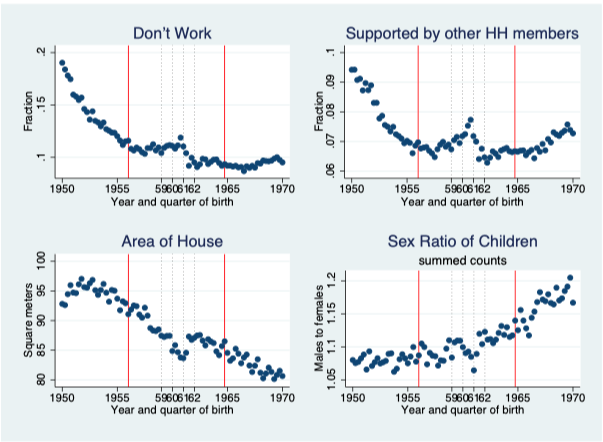
\includegraphics[width=0.9\linewidth]{figure5}
            \end{minipage}
           
            \column{0.4\textwidth} % remember add this to the other clumn
           	\begin{minipage}[c][0.4\textheight][c]{\linewidth}
            2000年的统计微观数据显示:在1960年前后出生的人,与同期预测相比有更差的社会经济产出。
            在1960年出生的人在2000年普查时特征:没有工作;受其他家庭成员支持;住在很小的地方;女童的父母
            \end{minipage}
    \end{columns}
\end{frame}

\begin{frame}
	\frametitle{Result:Regression Results}
	$$y_{it}=\beta_0+\theta~awdr_t+\beta_1YOB+\beta_2YOB^2+\beta_3YOB^3+\lambda_{province}+\varepsilon_{it}$$
	$y_{it}$代表t时期出生的i个体的结果变量,$awdr_t$表示按出生年份和出生月份计算的总加权死亡率;$YOB$出生年份,加入平方和立方项控制非线形趋势(图五的四幅图);$\lambda_{province}$省的虚拟变量,由于出生月份存在明显的内生性,所以不包括月份的虚拟变量
\end{frame}


\begin{frame}
\frametitle{Result:Regression Results}
	\begin{columns}
            \column{0.6\textwidth}
            \begin{minipage}[c][0.4\textheight][c]{\linewidth}
                \centering
                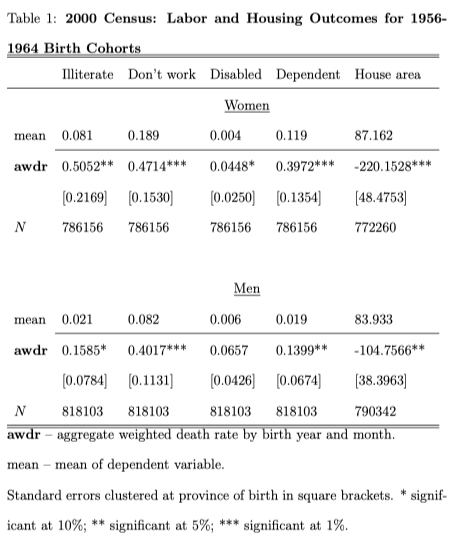
\includegraphics[width=0.9\linewidth]{table1}
            \end{minipage}
           
            \column{0.4\textwidth} % remember add this to the other clumn
           	\begin{minipage}[c][0.4\textheight][c]{\linewidth}
            Greater famine intensity is associated with a higher likelihood of being illiterate and not working.\\awdr提高1.2个百分点,意味着:饥荒经历的女性有$0.502*0.012/0.081=7.5\%$的可能性是文盲,但是这个普查的数据没有其他直接的关于收入的数据
            \end{minipage}
    \end{columns}
\end{frame}

\begin{frame}
\frametitle{Result:Regression Results}
	\begin{columns}
            \column{0.5\textwidth}
            \begin{minipage}[c][0.4\textheight][c]{\linewidth}
                \centering
                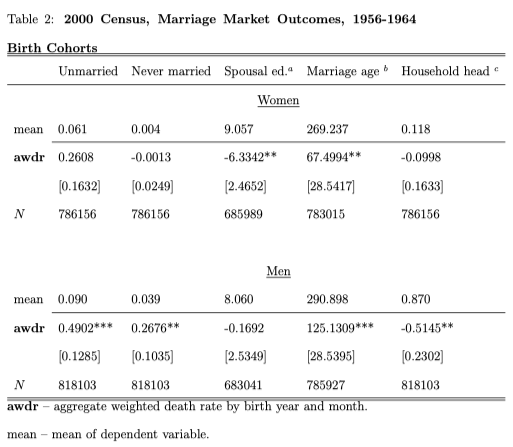
\includegraphics[width=1\linewidth]{table2}
            \end{minipage}
           
            \column{0.5\textwidth} % remember add this to the other clumn
           	\begin{minipage}[c][0.4\textheight][c]{\linewidth}
            表2主要研究对于婚姻市场的影响:对于女性而言不显著,但是女性更易的伴侣通常的教育程度更低,但是男性更易受到影响:未婚等,结婚年龄的影响,主要解释:婚姻市场挤压
            \end{minipage}
    \end{columns}
\end{frame}

\begin{frame}
\frametitle{Result:Regression Results}
	\begin{columns}
            \column{0.5\textwidth}
            \begin{minipage}[c][0.4\textheight][c]{\linewidth}
                \centering
                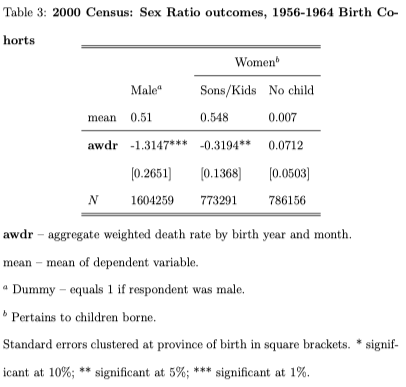
\includegraphics[width=1\linewidth]{table3}
            \end{minipage}
           
            \column{0.5\textwidth} % remember add this to the other clumn
           	\begin{minipage}[c][0.4\textheight][c]{\linewidth}
            男性死亡率提高,母亲经历过饥荒的越严重,后代中女性更多,因此需要香港数据进行验证
            \end{minipage}
    \end{columns}
\end{frame}

\begin{frame}
	\frametitle{Result:Geographic variation in Famine intensity}
    将饥荒的地域差异控制住,研究出生队列间的差异,这样会降低未来生活中其他因素与特定年龄混杂的可能性
$$y_{it}=\beta_0+\theta~wdr_t+\gamma_{yob}+\lambda_{province}+\varepsilon_{itj}$$
\end{frame}

\begin{frame}
\frametitle{Result:Geographic variation in Famine intensity}
    \begin{columns}
            \column{0.5\textwidth}
            \begin{minipage}[c][0.4\textheight][c]{\linewidth}
                \centering
                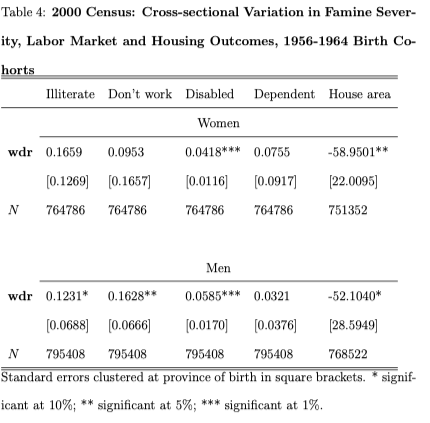
\includegraphics[width=1\linewidth]{table4}
            \end{minipage}
           
            \column{0.5\textwidth} % remember add this to the other clumn
            \begin{minipage}[c][0.4\textheight][c]{\linewidth}
            Table 4 shows that local famine severity indeed corresponds to the magnitude of damage in Census outcomes. Women born in high-Famine areas had larger increases in disability rates and larger reductions in house sizes. For men, differences in literacy, work status, disability, and house size correspond to Famine severity in the expected direction.
            \end{minipage}
    \end{columns}
\end{frame}


\begin{frame}
\frametitle{Result:Geographic variation in Famine intensity}
    \begin{columns}
            \column{0.5\textwidth}
            \begin{minipage}[c][0.4\textheight][c]{\linewidth}
                \centering
                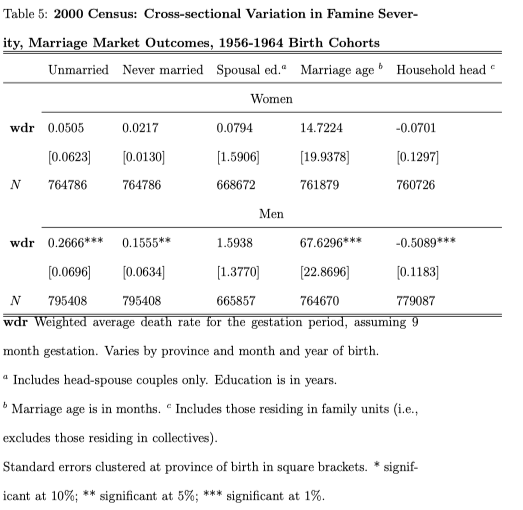
\includegraphics[width=1\linewidth]{table5}
            \end{minipage}
           
            \column{0.5\textwidth} % remember add this to the other clumn
            \begin{minipage}[c][0.4\textheight][c]{\linewidth}
            Men from high-Famine areas were less likely to be married (3.5\%), more likely to never have married (5\%), married older (.8 months), and were less likely to head their households (.7\%) (Table 5). For women, the point estimates have the expected signs, but are not statistically significant.
            \end{minipage}
    \end{columns}
\end{frame}

\begin{frame}
\frametitle{Result:Geographic variation in Famine intensity}
    \begin{columns}
            \column{0.5\textwidth}
            \begin{minipage}[c][0.4\textheight][c]{\linewidth}
                \centering
                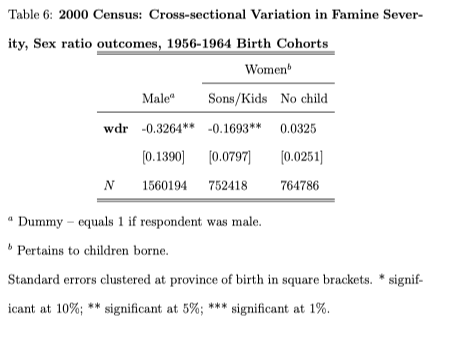
\includegraphics[width=1\linewidth]{table6}
            \end{minipage}
           
            \column{0.5\textwidth} % remember add this to the other clumn
            \begin{minipage}[c][0.4\textheight][c]{\linewidth}
            Table 6 shows that coefficients for the sex ratio are significant in the expected direction, but roughly one-third the size of the corresponding estimates in Table 3.
            \end{minipage}
    \end{columns}
\end{frame}

\begin{frame}
	\frametitle{Result:Potential Biases}
   \textcolor{red}{这没看懂}
   \\ 饥荒提高死亡率的同时也降低了出生率,2000年的普查数据显示经历过饥荒的人群比相近队列人群要少大约25-50\%,饥荒造成的死亡是负面的,那么对幸存者所受损害估计的偏误是向下的。
\end{frame}

\begin{frame}
	\frametitle{Result:Birth Outcomes in Hong Kong}
香港的数据提供了一个很好的对照组,当时政府严格禁止向外移民,但是在1962年相当大一部分人逃往香港,难民中有内地出生的孩子。饥荒期间或者饥荒以后从大陆迁徙到香港的群体,提供了很好的对照:迁往香港的群体与香港本地出生的人。
\end{frame}



\begin{frame}
\frametitle{Result:Birth Outcomes in Hong Kong}
    \begin{columns}
            \column{0.5\textwidth}
            \begin{minipage}[c][0.4\textheight][c]{\linewidth}
                \centering
                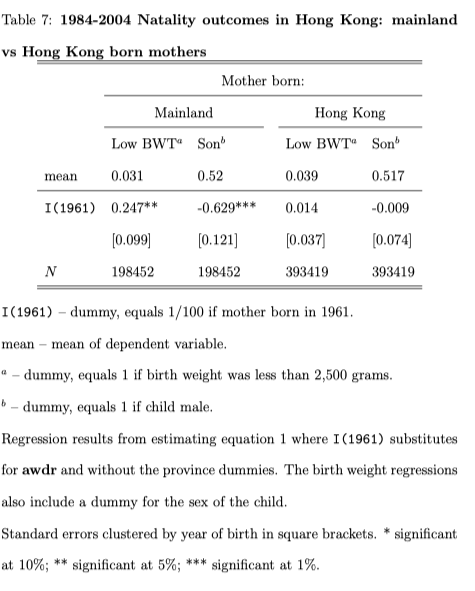
\includegraphics[width=1\linewidth]{table7}
            \end{minipage}
           
            \column{0.5\textwidth} % remember add this to the other clumn
            \begin{minipage}[c][0.4\textheight][c]{\linewidth}
            We find that mothers born in 1961 were 8\%= (0.247/0.030) more likely to give birth to a child of low birth weight (less than 2,500 grams) and 1.2\% (0.00629/0.52) less likely to give birth to a son than mothers born in adjacent years (Table 7).
            \end{minipage}
    \end{columns}
\end{frame}

\begin{frame}
    \frametitle{Summary and Discussion}
Higher Famine intensity was associated with greater risk of being illiterate, out of the labor force, marrying later (men), and marrying spouses with less education (women)
\\ Perhaps the most intriguing result is that Famine exposure lowered the sex ratio of not only the first but also the second generation.
\\ 文章的贡献在于这篇文章是第一篇准实验研究来给Trivers-Willard 提供证据,也是第一篇产妇营养状况对性别比的代际“回声”的研究
\end{frame}

\begin{frame}
	\frametitle{思考}
	父母经历过饥荒对于孩子的影响,这样数据会很丰富,也是个很好的研究点
	\\这篇文章是NBER的working paper但是却一直没发表。
\end{frame}


\end{document}


